\chapter{Disintermediation of Inter-Blockchain Transactions\label{cha:chapter4}}

Different versions of peer-to-peer electronic cash exist as data represented by separate blockchains. 
Payments between such systems using different ledgers cannot be sent directly from one party to another without going through a financial institution.
Bitcoin's utility is limited to intra-blockchain transactions.
The benefits of peer-to-peer electronic cash are lost if a trusted third party is required to execute \textit{inter}-blockchain transactions.
We propose a solution to the inter-blockchain transaction problem using the same fundamental principles underlying Bitcoin. 
The protocol is described by the \"{U}berledger framework, a hierarchical meta-blockchain layer that encapsulates information regarding the fidelity of peer-to-peer transaction facilitators. 

\section{Introduction}

In the world prior to the introduction of \emph{Bitcoin} no peer-to-peer version of electronic cash had managed to solve the problem of double-spending.  
Nakamoto in \cite{satoshi2008bitcoin} described the state of the art whereby a common solution had been to \enquote{introduce a trusted central authority, or mint, that checks every transaction for double spending... The problem with this solution is that the fate of the entire money system depends on the company running the mint, with every transaction having to go through them, just like a bank}. 

Bitcoin is an effective mechanism to circumvent dependence on a trusted central authority.
However, we have borne witness to the hydralike re-emergence of this phenomenon in the form of exchanges \textit{between} cryptocurrency systems.
For instance to transfer \euro100.00 of value between the cryptocurrencies Bitcoin (BTC) and \emph{Ethereum} (ETH) it is generally necessary to employ the services of an exchange such as \emph{Bitfinex}\footnote{ \texttt{www.bitfinex.com}}.

In this chapter we propose a framework that utilizes the same fundamental principles as Bitcoin.
Bitcoin disintermediates the exchange of value amongst participants on a common blockchain system.
We want to disintermediate transactions between individuals who have accounts on \textit{disjoint} blockchains, but nevertheless want to exchange value with each other. 
In the decentralized constellation of cryptocurrencies the focal points of centripetal force are digital currency exchangers. 
Centralized processes are susceptible to developing into single points of failure, a feature that resilient networks seek to minimize.
Digital currency exchangers provide primarily two services, they transfer value in digital currencies for fiat money, or different digital currencies.
We demonstrate that the interchange of value between different digital currencies is a task that can be performed with high fidelity in the absence of trusted third party exchangers through the use of a hierarchical meta-blockchain layer. 

\begin{figure}
\centering
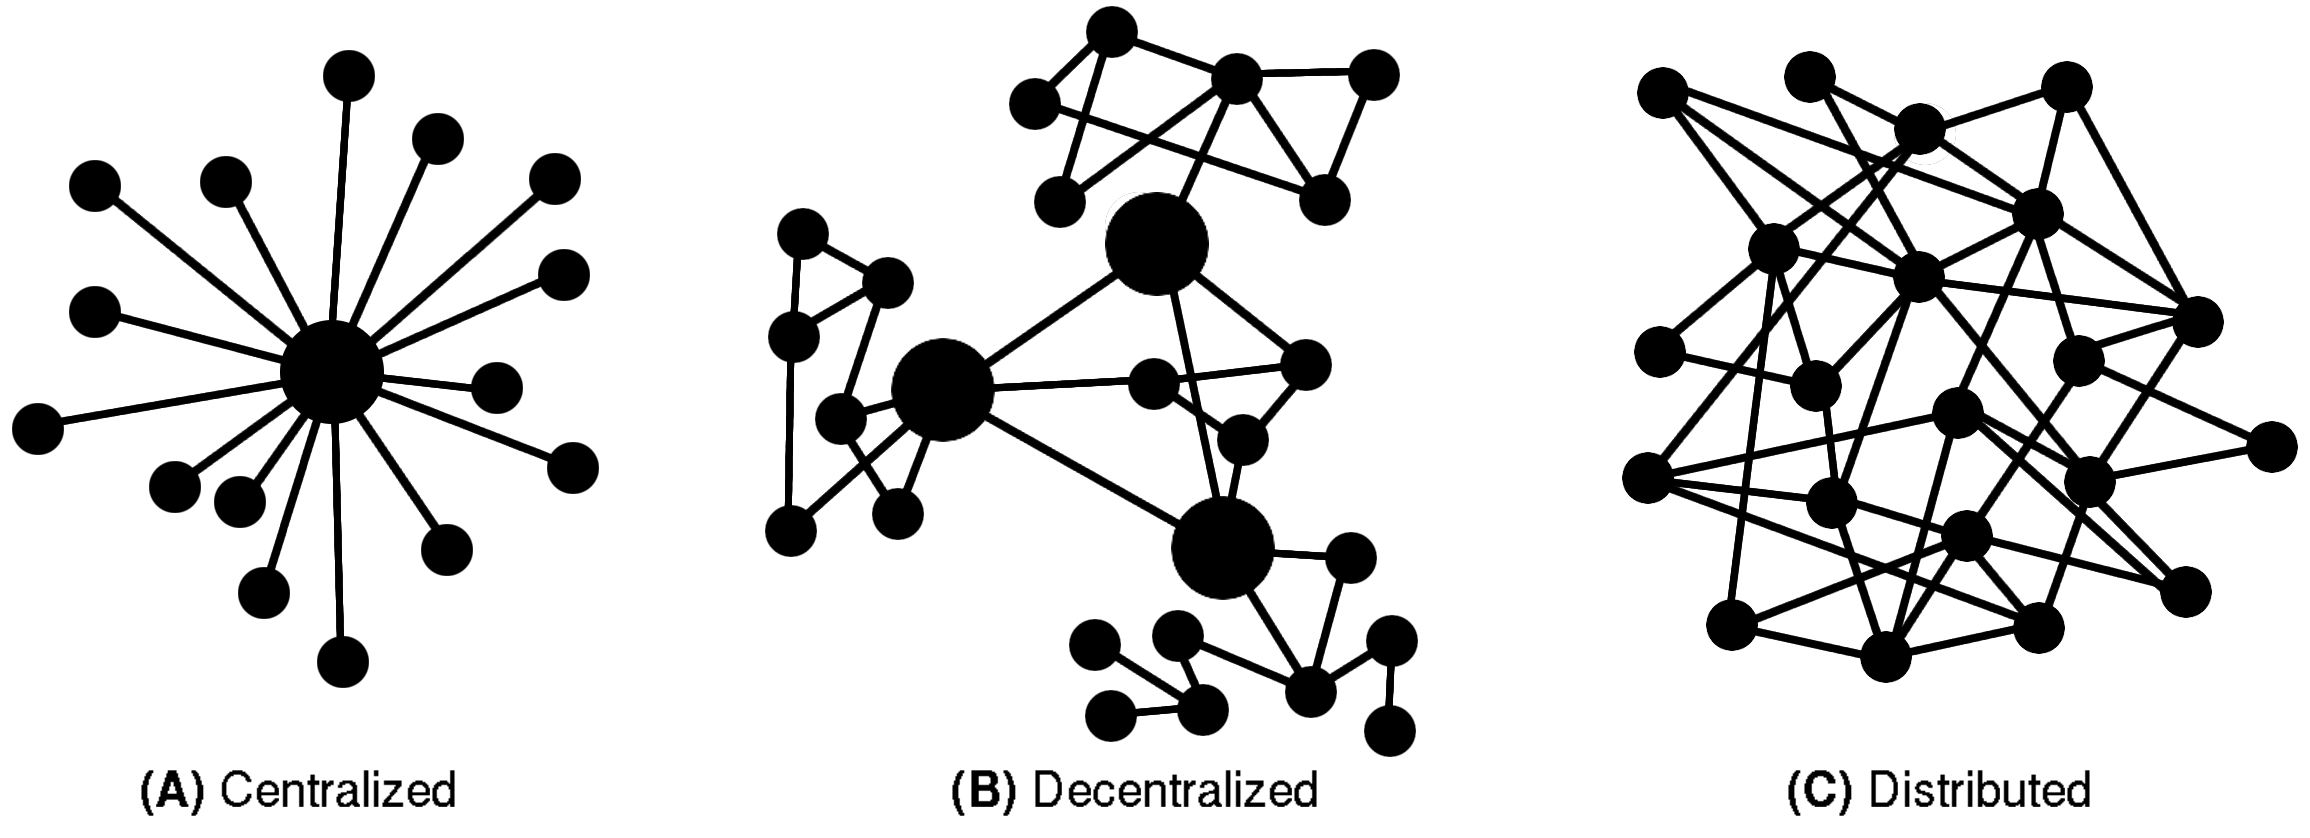
\includegraphics[width=0.5\textwidth]{Figure_1__0}
\caption{Network Topologies}
\end{figure}

\section{The Exchange Model}

On the $2^{nd}$ of August 2016 a highly trafficked digital currency exchange reported a heist of \$72,000,000 USD~\cite{baldwin_2016}. 
This is merely one episode in a history of criminal negligence or malfeasance going back to Mt. Gox (the infamous exchange responsible for the loss of \$460,000,000 in customer funds \cite{wire}) and beyond. 
Accordingly there is a strong interest in viable alternatives to transferring information, viz. value, between disparate blockchain systems independent from such central authorities.

Reliance on exchangers to move value between blockchain systems is a policy that suffers from the \enquote{inherent weaknesses of the trust based model}~\cite{satoshi2008bitcoin}.
Cryptocurrency users who have interacted with an exchange will be familiar with the stringent regime of know your customer (KYC) and will have had direct experience with exchanges \enquote{wary of their customers, hassling them for more information than they would otherwise need}~\cite{satoshi2008bitcoin}. 
As originally envisioned by Nakamoto in \cite{satoshi2008bitcoin} our framework is engineered to \enquote{allow online payments to be sent directly from one party to another without going through a financial institution}.

\begin{figure}
\centering
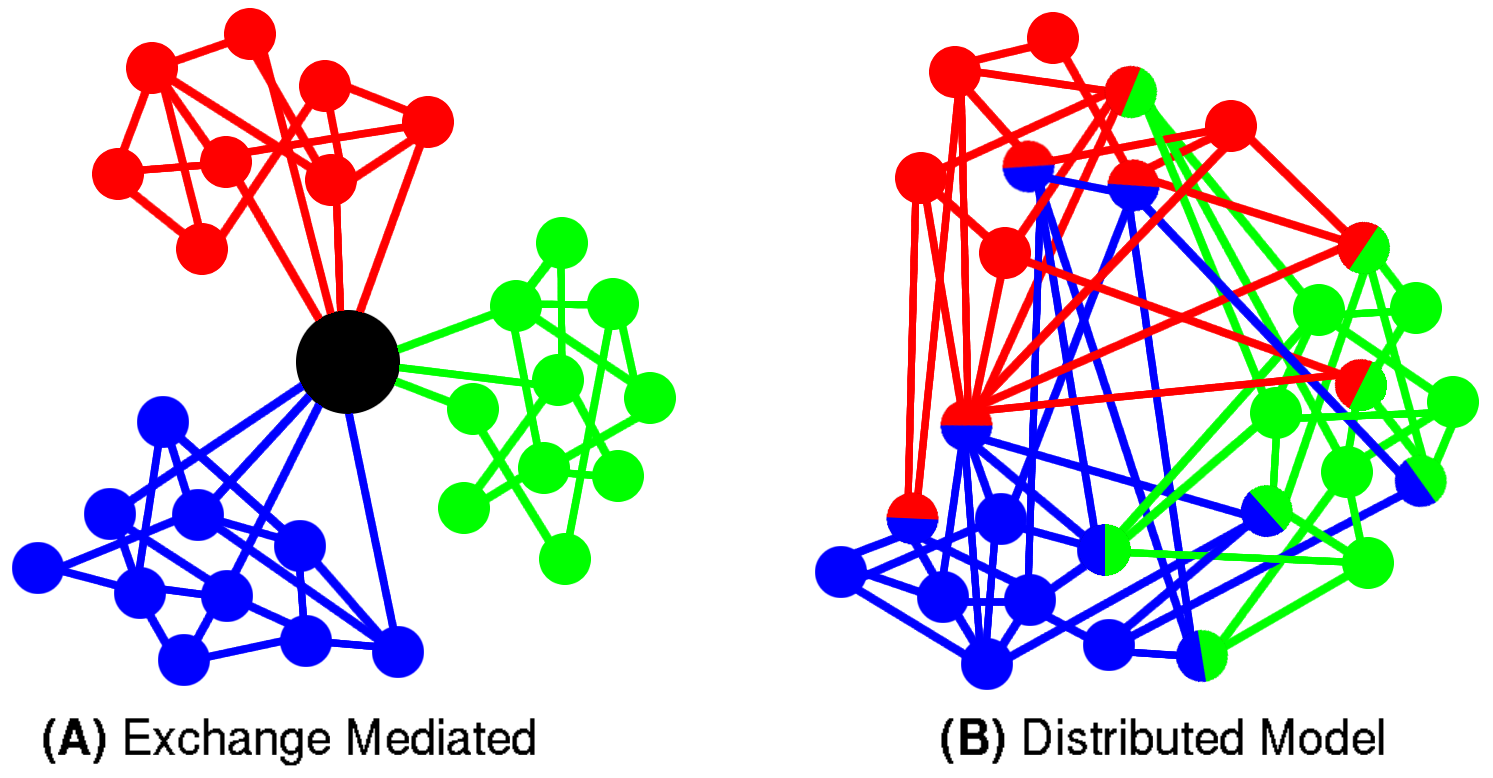
\includegraphics[width=0.5\textwidth]{Figure_2__1}
\caption{Inter-Blockchain Value Transmission}
\end{figure}

\section{Analogous Initiatives}

It has been shown by Thomas \& Schwartz in \cite{hope2016interledger} that protocols whereby a subset of network participants (with accounts on two distinct blockchains) is employed to act as \enquote{connectors and notaries}, i.e. facilitators of a transaction between ledgers, are feasible so long as the subset is sufficiently large to ensure that Byzantine actors can be readily identified ($\mathpzc{n}$ $\geq$ 3$\mathpzc{f}$+1). 

One design feature of the system described in \cite{hope2016interledger} is an ephemeral aggregation of transaction facilitators, such that \enquote{[facilitators] are organized in ad-hoc groups for each payment}.
This arrangement preserves the integrity of the funds involved in the transaction, either they are correctly allocated or the transaction is forfeit.
However information regarding the integrity of each node is not preserved in a publicly available repository of information, such as a blockchain, where it could be put to use in future transactions.  

In contrast to \cite{hope2016interledger} we seek to indelibly preserve all information regarding the successful (or unsuccessful) outcome of the transaction and the behaviour of constituent parties. 
The procedure sketched in Figure 4.3.


\section{Framework Architecture}

We introduce the \"{U}berledger framework\footnote{ \texttt{www.uberledger.io}}. 
It is a hierarchical blockchain model based on the following proposition:  

\theoremstyle{definition}
\begin{definition}{(\"{U}berledger)}
In the transference of value between two disjoint consensus networks the sequentiality of transactions cannot be preserved in the absence of an additional meta consensus network.
\end{definition}

Careful examination of Nakamoto's protocol in \cite{satoshi2008bitcoin} yields a strict sequentiality indicated by timestamps as the crux of the cryptocurrency system. 
We take timestampedness to mean that each transaction ($\mathpzc{t_i}$) is part of a linearly ordered list of transactions ($\mathpzc{T}=(t_1,\dots,t_n)$).
In our model consensus network is equivalent to blockchain, as defined by Kiayias et al. in \cite{garay2015bitcoin}. 

\begin{figure}
\centering
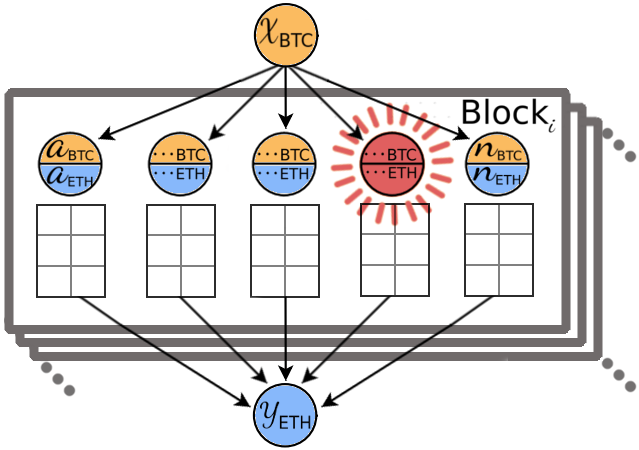
\includegraphics[width=0.5\textwidth]{Figure_3__0}
\caption{Disintermediated Inter-Blockchain Transaction}
\end{figure}

\section{Design Considerations}

\subsection{Incentive Structure}
The incentive structure that motivates the continued maintenance of a resilient blockchain is critical, as the undertaking is costly. 
Honest participants of the \"{U}berledger framework stand to be remunerated in proportion to their ability to attract transaction fees for their services.

\subsection{Data Representation}
Transactions are naturally represented in the form of a 3-tuple ($\mathpzc{P_1}$, $\mathpzc{a}$, $\mathpzc{P_2}$), where $\mathpzc{P_1}$ and $\mathpzc{P_2}$ are the transacting parties and $\mathpzc{a}$ is the article of trade. 
Accordingly, we employ the RDF data model and encapsulate salient transaction information in the form of a graph, as demonstrated in Figure 4. 
To define data in the form of a graph it is necessary to employ a schema.
For this purpose we have adapted the blockchain ontology with dynamic extensibility (BLONDiE)\footnote{\texttt{www.github.com/EIS-Bonn/BLONDiE}}.

This model ensures that a wide range of disparate data resources, e.g. multiple accounts across different blockchains, unique username, reputation information, and cryptographic keys, are rendered in a standardized and universally accessible format adhering to the W3C principles of linked open data.

\subsection{Participant Evaluation}
Insofar as the integrity of nodes in the framework exists as a matter of public record we adapt the design considerations in \cite{kamvar2003eigentrust} to serve as fundamental benchmarks of our peer-to-peer reputation system.
As such the protocol is: 
\begin{enumerate}
  \item Self-policing. 
  \item Anonymity maintaining.
  \item Negatively biased to newcomers.
  \item Minimal in overhead (i.e. computation, infrastructure, storage, and message complexity).
  \item Robust to malicious coordinated collectives.
\end{enumerate}

\section{Results}
The balkanization of the cryptocurrency ecosystem is a phenomenon that is enforced by the business model of the exchanges that seek to exploit their control over channels into and out of different blockchains inhibiting those interested in experimentation on new platforms. Such a climate stifles the ability to assess innovative features and challenge one's understanding of novel techniques. 
Our framework is engineered to redress such toll roads on the highway of creative endeavour.
\"{U}berledger is an open source initiative that seeks to engender an environment of free creative development.

\begin{figure}
\centering
\includegraphics[width=0.5\textwidth]{Facilitator_Graph}
\caption{Transaction Data Model}
\end{figure}


\section{Timestamp Hacking}

Any carnival conjuror can attest that once an audience learns the science behind the way in which a trick is performed, the luster quickly fades. 
The eminent futurist Sir Arthur Charles Clarke is credited with the observation that ``any sufficiently advanced technology is indistinguishable from magic''. 
Of late there is a profusion of hype in circulation about a seemingly magical data structure called a ``Blockchain''. 

Illusionists like Harry Houdini and his ilk can be a great source of entertainment, but when the trick involves a disappearing act on customer confidence, something is amiss. You might have heard that one of the properties a Blockchain possesses is the ability to ``prove certain data exists at a certain moment of time'' or that it somehow ``provides proof that some data existed at a specific tim''. 
The problem with these claims is that they are demonstrably false. 

\subsection*{Look to the Blockchain}

To prove this assertion we need look no further than the publically available Bitcoin Blockchain itself. 
Observe the sequence of blocks, and their associated timestamps, from 145044 to 145048.

\begin{itemize}
\item \texttt{145044: 2011-09-12 15:46:39}
\item \texttt{145045: 2011-09-12 16:05:07}
\item \texttt{145046: 2011-09-12 16:00:05} \\(\textit{Occurs about five minutes before the prior block})
\item \texttt{145047: 2011-09-12 15:53:36} \\(\textit{About seven & about twelve minutes before two prior blocks})
\item \texttt{145048: 2011-09-12 16:04:06} \\(\textit{After two prior blocks but still before} \texttt{145045})
\end{itemize}

We see here that the timestamp of the blocks is not monotonically increasing. 
To understand why, it's necessary for us to have a basic understanding of distributed computing systems, one of the elementary characteristics of which is the lack of a global clock. 
The time adjustment algorithm has even been called the most obvious possible weakness in the Bitcoin protocol.

\subsection*{Why don't the timestamps in the Blockchain always increase?}

It would behove those interested in Blockchain timestamping to consult the Bitcoin wiki for a more informed understanding of how timestamping is applied in this system:

\begin{displayquote}
``A timestamp is accepted as valid if it is greater than the median timestamp of the previous 11 blocks, and less than the network-adjusted time + two hours. `Network-adjusted time' is the median of the timestamps returned by all nodes connected to you.

Whenever a node connects to another node, it gets a UTC timestamp from it, and stores its offset from node-local UTC. The network-adjusted time is then the node-local UTC plus the median offset from all connected nodes. Network time is never adjusted more than 70 minutes from local system time, however''. 
\end{displayquote}

This implies an inherent margin of imprecision. When considering allowances made for anomalies such as daylight savings time and the potential for attacks against the network by malicious actors we quickly see that we need a more nuanced understanding of what timestamping in a Blockchain actually implies. And what it does not.

\subsection*{Timestamp hacking}

One reason that certain parties have an interest in knowingly contributing false timestamps to the network involves the way rewards are distributed according to the Bitcoin protocol. The difficulty of the ``cryptographic puzzle'' that miners are attempting to solve is configured to readjust its difficulty about every two weeks. If miners can fake their timestamps they can make it appear that the network is less powerful than in fact it really is, thus making the puzzle easier and potentially generating higher returns. Additional incentives include denial-of-service attacks against target nodes and in extraordinary cases even double-spend attacks.

\subsection*{Overview}

When one really starts to consider the meaning of time the subject quickly becomes philosophical. 
Spacetime describes a mathematical model that combines space and time into a single interwoven continuum based on the theories of special and general relativity first discovered by Albert Einstein. 
For purposes of time telling in our daily lives we seldom need to grapple with such principles. 
There are some truly impressive applications of blockchain technology. 
For better or worse, precision timestamping is not one of them.

